\chapter{Conceptual Tools}

% some notes on notation and a glossary of frequently used terms
\section{Conceptual Tools for Understanding Bootstrap Percolation}

As outlined above, it appears that lethal sets in grid graphs adhere to certain fixed rules. We examine these rules here, and explain why they are necessary and helpful for understanding the problem of bootstrap percolation.

\subsection{Integrality of bounds}

Not all grids have integral surface area bounds. We refer to such grids as \emph{non-divisibility cases}. The non-divisibility cases for three-dimensional grids where $r=3$ are illustrated in red in Table \ref{tab:integral_bounds}. 

Percolation in non-divisible grids is inefficient in one of two ways: either each vertex in $A_0$ contributes, on average, less than $2d$ units to the final surface area, or at some time-step $i$, there exists a vertex $v \in V \setminus A_i$ such that $N_{A_i}(v) > r$. In the first case, the inefficiency is a consequence of two adjacent vertices in $A_0$; heuristically, we may view this as poor distribution of infection across the grid. In the second case, the inefficiency results from excessive infection in a particular region; a vertex is over-exposed. 

It is insightful to consider this behavior in the context of Theorem \ref{thm:torus_lb}. Instead of thinking of $m_{IH}$ at the number of edges between $I$ and $H$, we shall consider it to represent the perimeter, or surface area, of the initial infection $I$. 
%In particular, the existence of adjacent vertices in $A_0$ corresponds precisely to inequality in $m_{IH} \leq 2d|I| - 2(ab+bc+ca)$, where $2(ab+bc+ca)$ is the surface area of the grid. 
%In these cases, we are guaranteed the existence of at least one cell that is infected by more than $r$ neighbors. This is a direct consequence of the surface area argument; since the final surface area of infection is non-integral and surface area is non-increasing

\begin{table}[]
\centering
\begin{subfigure}{0.3\textwidth}
	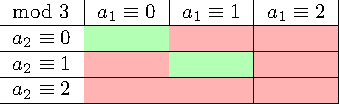
\includegraphics[width=\textwidth]{tables/1/integral_bounds_thickness_1.pdf}
	\caption{$a_3 \equiv 1 \pmod 3$}
	\label{tab:integral_bounds_a}
\end{subfigure} \hfill%
\begin{subfigure}{0.3\textwidth}
	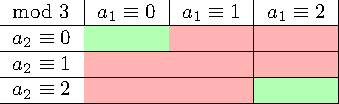
\includegraphics[width=\textwidth]{tables/1/integral_bounds_thickness_2.pdf}
	\caption{$a_3 \equiv 2 \pmod 3$}
	\label{tab:integral_bounds_b}
\end{subfigure} \hfill%
\begin{subfigure}{0.3\textwidth}
	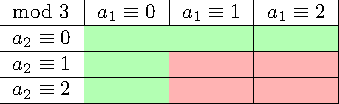
\includegraphics[width=\textwidth]{tables/1/integral_bounds_thickness_3.pdf}
	\caption{$a_3 \equiv 0 \pmod 3$}
	\label{tab:integral_bounds_c}
\end{subfigure}
\caption{Integrality of grids by congruence class. Green indicates integral surface area bound.}
\label{tab:integral_bounds}
\end{table} 

\subsection{A different characterization}

We shall find it useful to think about the problem of bootstrap percolation in terms of the graph induced by the set of uninfected vertices $V \setminus A_i$ at some time-step $t_i$. 

\subsection{Attributes of $G[V \setminus A]$}

No cycles, no paths between opposite faces. Reference to Benevides.

\subsection{The lower bound}

Let us reconsider the our proof of the lower bound in this new framework. 

\subsection{Surface area, optimality, trees, and components}

The surface area bound is not always integral. In cases where it is not, this sub-optimality can be traced to a particular time-step where an uninfected cell is infected by more than $r$ neighbors. The proof of the lower bound on the torus considers the number of components in $T[V \setminus A]$, as each such component necessarily collapses in on a vertex where this occurs. In the grid, this circumstance can be avoided by permitting components to abut the perimeter. What is the relationship here?

\subsection{The bipartition (and when to violate it)}

Discuss the heuristic of placing infections on one side of the bipartition and when this technique fails. 

\subsection{A potentially interesting proof framework}

A discussion on the broad structure of the proof of the lower bound on the torus as presented in Benevides. Note that this proof relies on a sequence of inequalities, and that two of these inequalities characterize precise conditions that are necessary for a set to be lethal. Discuss how the proof might change as a function of the dimension of the grid. 
